\section{Прерывания и их обработка: верхняя и нижняя половины}

Одной из самых ответственных функций ядра любой операционной системы является управление аппаратными устройствами, которые подключены
к вычислительной машине. 

Частью этой работы является необходимость взаимодействия с отдельными устройствами машины. Поскольку процессоры вычислительной машины обычно работают во много раз быстрее, чем оборудование, с которым они должны взаимодействовать, то с точки зрения ядра получается неэффективным отправлять запросы и тратить время на ожидание ответа от существенно более медленного устройства. 

Как же может процессор работать с аппаратными устройствами и не замедлять при этом работу системы в целом? Лучшим решением будет создание механизма, который позволит подать сигнал ядру о том, что нужно уделить внимание оборудованию. Такой механизм называется \textit{прерыванием (interrupt)}. В этой главе мы рассмотрим прерывания и способы их обработки в ядре, а также специальные функции, которые называются \textit{обработчиками прерываний (interrupt handlers)}.

\subsection{Прерывания}
Прерывания позволяют аппаратным устройствам послать сигнал процессору. Физически прерывания вызываются специальными электрическими сигналами, которые генерируются устройствами и направляются на входные контакты микросхемы \textit{контроллера прерываний (interrupt controller)}

Сигналы прерывания, поступающие от устройств, часто называют \textit{линиями запросов на прерывание (interrupt request lines, IRQ)}. Каждой линии IRQ назначается соответствующий номер, который является восьмиразрядным двоичным числом

\subsection{Обработчики прерываний}

Функция, которую запускает ядро в ответ на поступление сигнала определенного прерывания, называется \textit{обработчиком прерывания (interrupt handler)}, или \textit{программой обслуживания прерывания (interrupt service routine)}. Каждому устройству, которое может генерировать прерывания, в ядре соответствует свой обработчик прерывания. Например, одна функция обрабатывает прерывание от системного таймера, а другая — прерывания, сгенерированные клавиатурой. Обработчик прерывания для определенного устройства является частью драйвера этого устройства — кода ядра, который управляет устройством.

В операционной системе Linux обработчики прерываний — это обычные функции, написанные на языке программирования C. Они должны соответствовать определенному
прототипу, чтобы ядро могло стандартным образом передавать информацию обработчику. Единственное, что отличает обработчики прерываний от других функций ядра, — это то, что они вызываются ядром в ответ на прерывание и выполняются в специальном контексте, именуемом \textit{контекстом прерывания (interrupt context)}. Этот специальный контекст иногда называют неделимым (atomic), поскольку код, выполняемый в нем, не может быть блокирован.

\subsection{Верхняя и нижняя половины}
Очевидно, требования о том, что обработчик прерывания должен выполняться как можно быстрее и при этом делать много работы, являются противоречивыми. В связи с этим процесс обработки прерываний разбивается на две части,
или половины. Обработчик прерывания относится к \textit{верхней половине (top half)}. Он запускается сразу после получения прерывания и выполняет только ту работу, которая критична к задержкам по времени, такую, как отправка подтверждения о получении прерывания или сброс аппаратного устройства. Работа, которую можно выполнить позже, откладывается до запуска \textit{нижней (или основной) половины (bottom half)}. Обработка нижней половины начинается позже, в более удобное время, когда все прерывания разрешены.

\subsection{Регистрация обработчика прерывания}
Драйвер может зарегистрировать обработчик прерывания, поступающего от заданной
линии IRQ следующим образом.

\begin{lstlisting}
#include <linux/interrupt.h>.

int request_irq(unsigned int irq,
 irq_handler_t handler,
 unsigned long flags,
 const char *name,
 void *dev)
 
\end{lstlisting}

Рассмотрим параметры подробней.

\begin{enumerate}
    \item\textit{irq}: указывает на занимаемый номер прерывания
    \item\textit{handler}: указатель на функцию обработчика прерывания, которая обслуживает данное прерывание
    \item\textit{flags}: может быть равным нулю или содержать битовую маску флагов, описанных в файле <linux/interrupt.h>
    \item\textit{name}: ASCII-строка, описывающая устройство, связанное с данным обработчиком прерывания
    \item\textit{dev}: используется в обработчиках прерываний, обслуживающих общие линии IRQ. При освобождении обработчика в параметре dev указывается уникальный идентификатор, который позволяет удалить только требуемый обработчик из заданной линии IRQ
    \item\textit{return value}: В случае успешного выполнения функция \code{request\_irq()} возвращает нулевое значение. Ненулевое значение свидетельствует о возникшей ошибке. В последнем случае обработчик прерывания не регистрируется.
\end{enumerate}

\subsection{Освобождение обработчика прерывания}
При выгрузке драйвера устройства из памяти компьютера необходимо отменить регистрацию обработчика прерывания и по возможности заблокировать линию IRQ. Для
этого вызывается приведенная ниже функция.
\begin{lstlisting}
void free_irq(unsigned int irq, void *dev)
\end{lstlisting}
Если указанная линия IRQ используется монопольно, то эта функция удаляет обработчик прерывания и блокирует линию IRQ. Если линия IRQ используется совместно с другими обработчиками прерываний, то удаляется обработчик, соответствующий параметру dev.

\subsection{Написание обработчика прерывания}
Рассмотрим настоящий обработчик прерывания, который используется в драйвере часов реального времени (real-time clock, RTC), находящегося в файле \code{drivers/char/rtc.c}

При загрузке драйвера устройства RTC вызывается функция \code{rtc\_init()} для инициализации драйвера:
\begin{lstlisting}
if (request_irq(rtc_irq, rtc_interrupt, IRQF_SHARED, "rtc", 
    (void*)&rtc_port)) {
  printk(KERN_ERR "rtc: cannot register IRQ %d\n", rtc_irq);
  return -EIO;
}
\end{lstlisting}

И сам обработчик прерывания:
\begin{lstlisting}
static irqreturn_t rtc_interrupt(int irq, void *dev)
{
 spin_lock(&rtc_lock);
 rtc_irq_data += 0x100;
 rtc_irq_data &= ~0xff;
 rtc_irq_data |= (CMOS_READ(RTC_INTR_FLAGS) & 0xF0);
 if (rtc_status & RTC_TIMER_ON)
 mod_timer(&rtc_irq_timer, jiffies + HZ/rtc_freq + 2*HZ/100);
 spin_unlock(&rtc_lock);

 spin_lock(&rtc_task_lock);
 if (rtc_callback)
 rtc_callback->func(rtc_callback->private_data);
 spin_unlock(&rtc_task_lock);
 wake_up_interruptible(&rtc_wait);
 kill_fasync(&rtc_async_queue, SIGIO, POLL_IN);
 return IRQ_HANDLED;
}
\end{lstlisting}

Эта функция вызывается всякий раз, когда система получает прерывание от устройства RTC. Прежде всего следует обратить внимание на вызовы функций спинблокировок: первая группа вызовов функций гарантирует, что к переменной \code{rtc\_irq\_data} не будет конкурентных обращений со стороны других процессоров на SMPмашине. Вторая группа вызовов функций защищает в аналогичной ситуации поля структуры \code{rtc\_callback}.

Переменная \code{rtc\_irq\_data} имеет тип \code{unsigned long}. В ней хранится информация
об устройстве RTC, которая обновляется при поступлении каждого прерывания и отражает состояние прерывания.
Далее, если запущен генератор периодических сигналов, обновляется значение системного таймера с помощью функции \code{mod\_timer()}.

В последней части кода, запускается функция обратного вызова, если таковая установлена. Драйвер RTC позволяет устанавливать функцию обратного вызова, которая может быть зарегистрирована из вне. В результате она будет запускаться при каждом прерывании, приходящем от устройства RTC.
В конце функция обработки прерывания возвращает значение \code{IRQ\_HANDLED}, чтобы
указать, что прерывание от данного устройства корректно обработано. Поскольку данный обработчик прерывания не поддерживает общих запросов на прерывание и в устройстве RTC не существует механизма, позволяющего обнаружить паразитные прерывания, этот обработчик всегда возвращает значение \code{IRQ\_HANDLED}.

\subsection{Контекст прерывания}
При выполнении обработчика прерывания ядро находится в контексте прерывания.
Напомним, что контекст процесса — это режим, в котором работает ядро, выполняя работу от имени процесса, например выполнение вызова системной функции или потока ядра.
В отличие от контекста процесса контекст прерывания не связан ни с одним процессом. Поскольку в контексте прерывания нет сопровождающего его процесса, этот контекст нельзя перевести в состояние ожидания. Дело в том, что тогда нарушилась бы работа системного планировщика: нельзя запланировать контекст, в котором нет задачи. Поэтому некоторые функции ядра не могут быть вызваны из контекста прерывания. Если функция может переводить процесс
в состояние ожидания, то ее нельзя вызывать в обработчике прерывания.

Контекст прерывания является критичным ко времени выполнения, поскольку на время обработки прерывания выполнение некоторого программного кода прекращается.
Код же самого обработчика прерывания должен быть простой и быстрый. Использование в нем циклов проверки состояния чего-либо (busy loop) крайне нежелательно, хотя и возможно. Всегда следует помнить, что обработчик прерывания прерывает работу некоторого кода (возможно, даже обработчика другой линии запроса на прерывание!). Максимально возможную часть работы необходимо изъять из обработчика прерывания и переложить на его нижнюю половину, которая выполняется в более подходящее время.


Во время конфигурации системы можно определить размер стека обработчика прерывания. Исторически так сложилось, что обработчик прерывания не имел собственного стека. Вместо этого он должен был использовать стек ядра прерванного процесса\footnote{В системе всегда выполняется какой-нибудь процесс. Если активных задач нет, то система переключается на выполнение \textit{холостой задачи (idle task)}}. Стандартный размер стека ядра составляет две страницы памяти, что обычно соответствует 8 Кбайт для 32-разрядных аппаратных платформ и 16 Кбайт — для 64-разрядных.

В ранних версиях ядер серии 2.6 была введена возможность уменьшить размер стека
ядра от двух до одной страницы памяти. Чтобы можно было работать со стеком уменьшенного размера, каждому обработчику прерывания выделили свой стек, отдельный для каждого процессора, размером в одну страницу памяти. Этот стек назвали \textit{стеком прерывания}. Хотя общий размер стека прерывания и равен половине первоначально размера совместно используемого стека,
тем не менее в результате выходит, что суммарный размер стека получается большим,
потому что теперь на каждый стек прерывания выделяется целая страница памяти.

Обработчик прерывания не должен зависеть от того, какие настройки стека используются и чему равен размер стека ядра. Поэтому всегда нужно использовать минимально возможное количество памяти в стеке.

\subsection{Система обработки прерывания и ее реализация}

Рассмотрим схему прохождения запроса прерывания, сгенерированного аппаратным устройством, по ядру системы.

\begin{figure}[h]
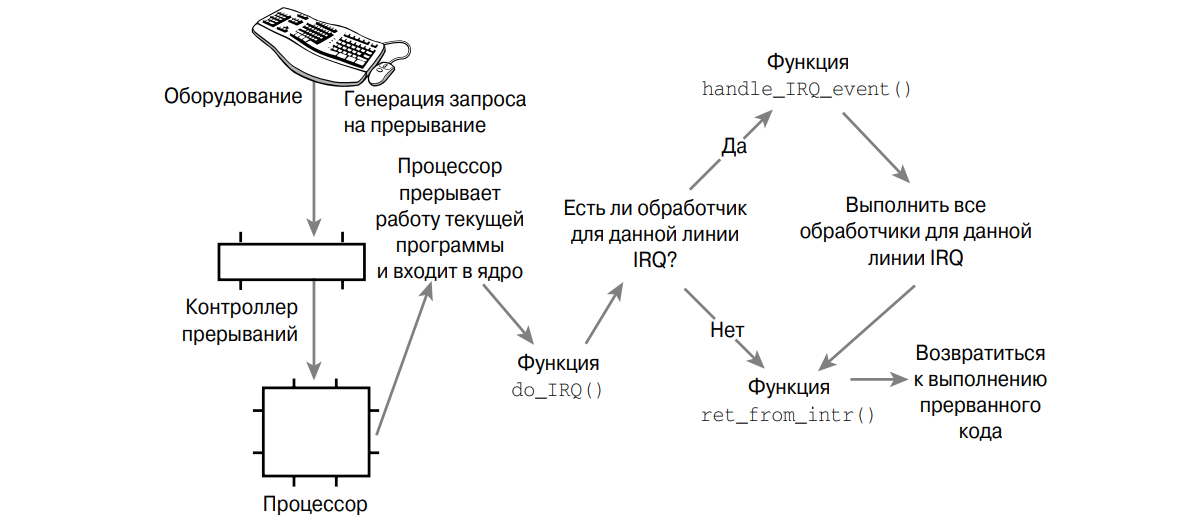
\includegraphics[width=\textwidth]{interruprions_handling.png}
\caption{Схема прохождения запроса прерывания}
\end{figure}

Устройство инициирует прерывание путем отправки электрического сигнала контроллеру прерываний по аппаратной шине. Если соответствующая линия запроса на прерывание (IRQ) не запрещена (линия может быть в данный момент времени замаскирована), то контроллер прерываний отправляет сигнал прерывания процессору. На большинстве аппаратных платформ это осуществляется путем подачи сигнала на специальный
вход микросхемы центрального процессора. Если прерывания в процессоре разрешены, то процессор завершает выполнение текущей машинной команды, запрещает прием новых прерываний, осуществляет переход на специальный предопределенный адрес в памяти и начинает выполнять программный
код, который находится по этому адресу. Этот предопределенный адрес памяти был заранее сконфигурирован ядром и является точкой входа в обработчики прерываний.

Для каждой линии IRQ в памяти машины предусмотрена своя уникальная точка входа. В точке входа сначала сохраняется в стеке значение номера прерывания и значения всех регистров процессора, которые относились к прерванной задаче. После этого ядро вызывает:

\begin{lstlisting}
unsigned int do_IRQ(struct pt_regs regs);
\end{lstlisting}

Далее в функции \code{do\_IRQ()} выполняется проверка, что для данной линии IRQ зарегистрирован корректный обработчик прерывания, что этот обработчик разрешен и не
выполняется в данный момент. Если все эти условия выполняются, то вызывается функция \code{handle\_IRQ\_event()}, определенная в файле \code{kernel/irq/handler.c}, которая запускает установленные для данной линии IRQ обработчики прерывания.

Функция \code{ret\_from\_intr()} и код входа в прерывание написаны на языке ассемблера. В этой функции проверяется, есть ли ожидающий запрос на перепланирование процессов. Если есть запрос на перепланирование и ядро должно передать управление в пространство пользователя (т.е. прерывание прервало работу пользовательского процесса), то вызывается функция \code{schedule()}. 
Если возврат производится в пространство ядра (т.е. прерывание прервало работу кода ядра), то функция \code{schedule()} вызывается, только если значение счетчика \code{preempt\_count} равно нулю. В противном случае код ядра не может быть безопасно вытеснен. После возврата из функции \code{schedule()} или если нет никакой ожидающей работы, восстанавливаются исходные значения регистров процессора и ядро продолжает свою работу там, где оно было прервано.

\subsection{Управление прерываниями}

В ядре Linux реализовано семейство интерфейсов для управления состояниями прерываний в машине. Эти интерфейсы позволяют запрещать прерывания для текущего
процессора или маскировать линию запроса на прерывание для всей машины. Все эти функции зависят от аппаратной платформы и находятся в файлах \code{<asm/system.h>} и \code{<asm/irq.h>}

\subsubsection{Запрещение и разрешение прерываний}

Для локального запрещения прерываний на текущем процессоре (и только на текущем) и последующего их разрешения можно использовать приведенный ниже код.

\begin{lstlisting}
unsigned long flags;
local_irq_save(flags);
/* Interruptions are forbidden */
local_irq_restore(flags); /* Restore initial state */
\end{lstlisting}

\subsubsection{Запрещение заданной линии IRQ}

В некоторых случаях может понадобиться запретить прерывание, поступающее от определенной линии IRQ для всей системы. Это называется \textit{маскированием линии запроса} на прерывание. Например, может потребоваться запретить прерывание, поступающее от некоторого устройства, перед изменением его состояния. Для этой цели в операционной системе Linux предусмотрены четыре интерфейса.

\begin{lstlisting}
void disable_irq(unsigned int irq);
void disable_irq_nosync(unsigned int irq);
void enable_irq(unsigned int irq);
void synchronize_irq(unsigned int irq);
\end{lstlisting}

\subsubsection{Методы управления прерываниями}

\begin{figure}[h]
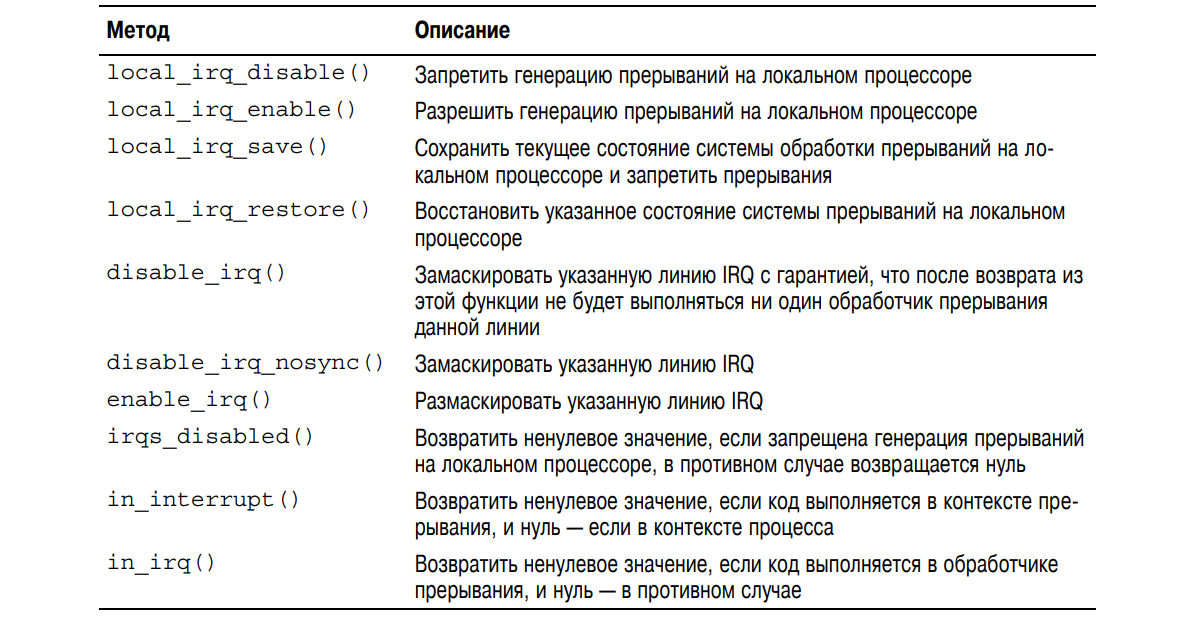
\includegraphics[width=\textwidth]{irq_control.png}
\caption{Методы управления прерываниями}
\end{figure}

\section{Нижняя половина обработчика и отложенные действия}

Хотя нет строгих правил по поводу того, как делить работу между верхней и нижней половинами обработчика прерываний, все же можно привести несколько полезных советов.

\begin{enumerate}
    \item Если работа критична по времени, то ее необходимо выполнять в обработчике прерывания
    \item Если работа связана с аппаратным обеспечением, то ее следует выполнить в обработчике прерывания
    \item Если для выполнения работы необходимо гарантировать, что другое прерывание (обычно с тем же номером) не прервет обработчик, то работу нужно выполнить в обработчике прерывания
    \item Всю остальную работу следует выполнять в нижней половине обработчика
\end{enumerate}

\subsection{Отложенные прерывания}

Обсуждение существующих методов построения нижних половин обработчиков прерываний начнем с механизма \textit{отложенных прерываний (softirq)}\footnote{Его код находится в файле \code{kernel/softirq.c}}. Сам по себе этот механизм напрямую используется редко, поскольку он положен в основу более общего механизма создания нижних половин обработчиков прерываний — тасклетов.

\subsubsection{Реализация механизма отложенных прерываний}

Отложенные прерывания определяются статически во время компиляции. В отличие от тасклетов, нельзя динамически зарегистрировать или удалить отложенное прерывание. Отложенные прерывания описываются с помощью структуры типа \code{softirq\_action}, которая определена в файле \code{<linux/interrupt.h>}:

\begin{lstlisting}
struct softirq_action {
 void (*action)(struct softirq_action *);
};
\end{lstlisting}

Массив, состоящий из 32 экземпляров этой структуры, определен в файле \textbf{kernel/softirq.c}.
\begin{lstlisting}
static struct softirq_action softirq_vec[NR_SOFTIRQS];
\end{lstlisting}
Каждое зарегистрированное отложенное прерывание соответствует одному элементу этого массива. Поэтому всего можно зарегистрировать \code{NR\_SOFTIRQS} отложенных прерываний.

\subsubsection{Обработчик отложенных прерываний}
Прототип обработчика отложенного прерывания, action:
\begin{lstlisting}
void softirq_handler(struct softirq_action *)
\end{lstlisting}

При выполнении в ядре этого обработчика отложенных прерываний запускается функция action, которой в качестве единственного аргумента передается указатель на соответствующую структуру типа \code{softirq\_action}. Например, если переменная \code{my\_softirq} содержит указатель на элемент массива \code{softirq\_vec}, то ядро вызовет функцию-обработчик соответствующего отложенного прерывания в следующем виде:
\begin{lstlisting}
my_softirq->action(my_softirq);
\end{lstlisting}

\subsubsection{Запуск отложенных прерываний}

Перед тем как зарегистрированное отложенное прерывание будет запущено, оно должно быть промаркировано. Этот процесс называется \textit{генерацией отложенного прерывания (rise softirq)}.
Проверка ожидающих выполнения обработчиков отложенных прерываний и их запуск осуществляется в перечисленных ниже случаях
\begin{enumerate}
    \item При возврате из обработчика аппаратного прерывания
    \item В контексте потока ядра ksoftirqd
    \item В любом коде ядра, в котором явно проверяются и запускаются ожидающие обработчики отложенных прерываний, как, например, это делается в сетевой подсистеме
\end{enumerate}

Независимо от метода вызова отложенного прерывания его выполнение осуществляется в функции \code{\_\_do\_softirq()}, которая вызывается из функции \code{do\_softirq()}.Если в системе есть ожидающие выполнения отложенные прерывания, то функция \code{\_\_do\_softirq()} в цикле проверяет их все и вызывает ожидающие обработчики. Рассмотрим упрощенный вариант самой важной части этой функции
\begin{lstlisting}
u32 pending;
pending = local_softirq_pending();
if (pending) {
  struct softirq_action *h;
  /* Reset bit mask of pending requests */
  set_softirq_pending(0);
  h = softirq_vec;
  do {
  if (pending & 1)
  h->action(h);
  h++;
  pending >>= 1;
  } while (pending);
}
\end{lstlisting}

Этот фрагмент кода является “сердцем” обработчика отложенных прерываний. В нем
проверяются и запускаются все ожидающие отложенные прерывания

\subsubsection{Примеры отложенных прерываний}

\begin{figure}[h]
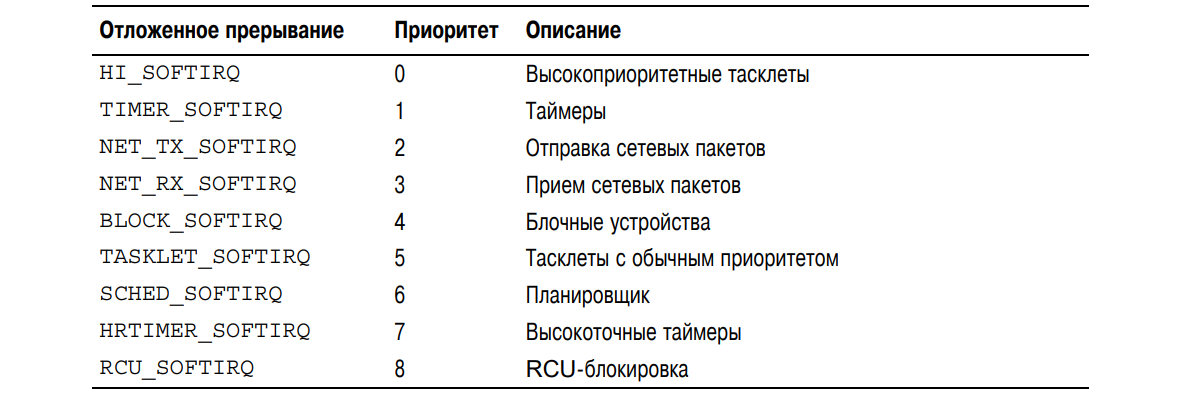
\includegraphics[width=\textwidth]{delayed_irq.png}
\caption{Список отложенных прерываний}
\end{figure}

\subsection{Тасклеты}

Тасклеты — это механизм построения нижних половин обработчиков прерываний на
основе механизма отложенных прерываний.

\subsubsection{Реализация тасклетов}
Поскольку тасклеты реализованы на основе отложенных прерываний, они также являются отложенными прерываниями. Как уже отмечалось выше, тасклеты представлены
двумя типами отложенных прерываний: \code{HI\_SOFTIRQ} и \code{TASKLET\_SOFTIRQ}. Единственная разница между ними в том, что тасклеты типа \code{HI\_SOFTIRQ} запускаются всегда раньше тасклетов типа \code{TASKLET\_SOFTIRQ}.

\subsubsection{Структуры тасклетов}
Тасклеты представляются в виде структуры \code{tasklet\_struct}. Каждый экземпляр структуры представляет собой уникальный тасклет. Эта структура определена в файле \code{<linux/interrupt.h>}:
\begin{lstlisting}
struct tasklet_struct {
  struct tasklet_struct *next; /* Pointer to the next tasklet in the list */
  unsigned long state; /* Tasklet's state */
  atomic_t count; /* Reference counter */
  void (*func)(unsigned long); /* Tasklet handler function */
  unsigned long data; /* Tasklet handler function argument */
};
\end{lstlisting}

\subsubsection{Планирование тасклетов на выполнение}

Запланированные (scheduled) на выполнение тасклеты (эквивалент сгенерированных отложенных прерываний) хранятся в двух структурах, определенных для каждого процессора: \code{tasklet\_vec} (для обычных тасклетов) и \code{tasklet\_hi\_vec} (для высокоприоритетных тасклетов). Каждая из этих структур представляет собой связанный список структур \code{tasklet\_struct}. Каждый экземпляр структуры \code{tasklet\_struct} представляет собой отдельный тасклет.

Тасклеты планируются на выполнение с помощью функций \code{tasklet\_schedule()} и \code{tasklet\_hi\_schedule()}, которым передается единственный аргумент — указатель на структуру \code{tasklet\_struct}.

\subsection{Очереди отложенных действий}

Очереди отложенных действий (work queue) — это еще один способ реализации отложенных операций. Очереди действий позволяют откладывать некоторые операции для последующего выполнения в потоке ядра. Данный тип нижних половин обработчиков всегда выполняется в контексте процесса и, как следствие, пользуется всеми преимуществами контекста процесса. Главное из них состоит в том, что этим процессом управляет системный планировщик, поэтому выполняющийся код может переходить в состояние ожидания.

\subsubsection{Структуры данных для представления рабочих потоков}
В самом общем случае подсистема очередей отложенных действий — это интерфейс для создания потоков ядра, выполняющих действия, которые кем-то были поставлены в очередь. Эти потоки ядра называются рабочими потоками (worker threads).

Рабочие потоки представляются с помощью структуры \code{workqueue\_struct}

\begin{lstlisting}
struct workqueue_struct {
  struct cpu_workqueue_struct cpu_wq[NR_CPUS];
  struct list_head list;
  const char *name;
  int singlethread;
  int freezeable;
  int rt;
};
\end{lstlisting}

Эта структура определена в файле kernel/workqueue.c. В ней содержится массив структур \code{cpu\_workqueue\_struct}, каждый элемент которого соответствует одному процессору в системе. Эта структура является основной и также определена в файле kernel/workqueue.c:

\begin{lstlisting}
struct cpu_workqueue_struct {
  spinlock_t lock;

  struct list_head worklist;
  wait_queue_head_t more_work;
  struct work_struct *current_struct;
  struct workqueue_struct *wq;
  task_t *thread;
};
\end{lstlisting}

\subsubsection{Структуры для представления отложенных действий}

Все рабочие потоки реализованы как обычные потоки ядра, которые выполняют функцию \code{worker\_thread()}. После начальной инициализации эта функция входит в бесконечный цикл и переходит в состояние ожидания. Когда какая-либо работа ставится в очередь, поток активизируется и выполняет ее. Когда в очереди не остается работы, которую нужно выполнить, поток снова переходит в состояние ожидания. Каждое действие представлено с помощью структуры \code{work\_struct}, определенной в файле <linux/workqueue.h>.
\begin{lstlisting}
struct work_struct {
  atomic_long_t data;
  struct list_head entry;
  work_func_t func;
};
\end{lstlisting}

Эти структуры объединены в связанный список, по одному списку на каждый тип очереди для каждого процессора.

\subsection{Блокировки между нижними половинами обработчиков}
Если имеются данные, которые могут совместно использоваться и в контексте прерывания, и в нижней половине обработчика, то перед обращением к ним нужно запретить прерывания и захватить соответствующую блокировку.


\subsubsection{Запрещение обработки нижних половин}
Обычно только одного запрещения обработки нижних половин недостаточно. Чаще всего для полной защиты совместно используемых данных нужно захватить соответствующую блокировку и запретить обработку нижних половин.

\begin{figure}[h]
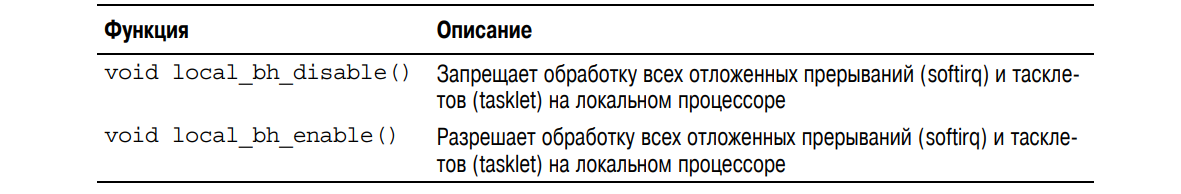
\includegraphics[width=\textwidth]{lock_delayed.png}
\caption{Функции управления обработкой нижних половин}
\end{figure}

Вызовы этих функций могут быть вложенными — при этом только последний вызов функции \code{local\_bh\_enable()} разрешает запуск нижних половин обработчиков прерываний. Например, при первом вызове функции \code{local\_bh\_disable()} запрещается выполнение отложенных прерываний на текущем процессоре. Если эта функция вызывается еще три раза, то выполнение отложенных прерываний на локальном процессоре будет запрещено. Их выполнение не будет разрешено до тех пор, пока функция \code{local\_bh\_enable()} не будет вызвана четыре раза.